\chapter{User Interface Konzept}
\section{Allgemeines und Funktionalität}
\begin{figure}[H]
    \centering
    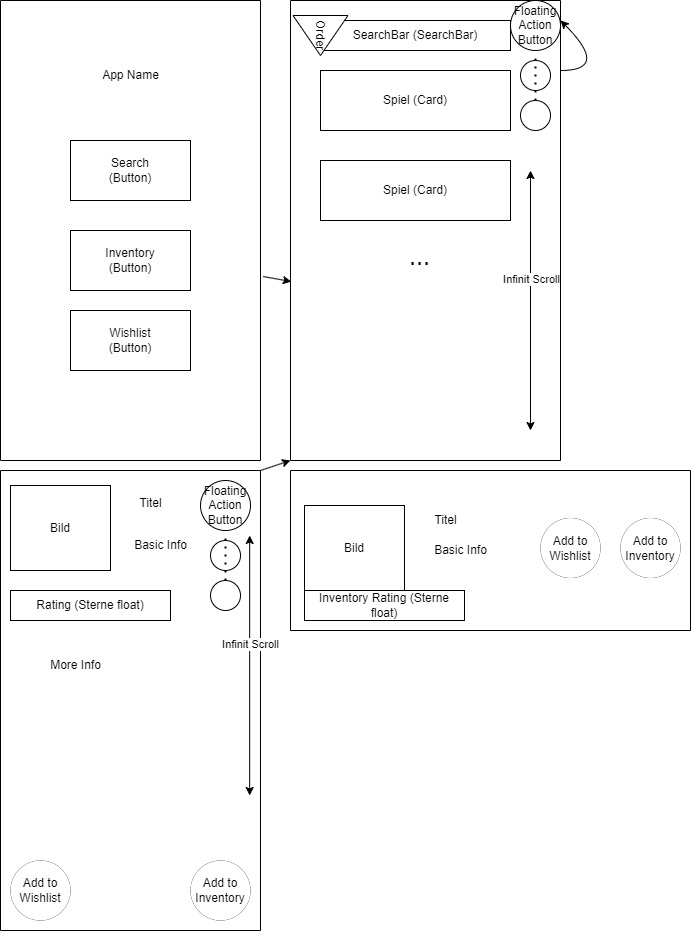
\includegraphics[width=0.6\textwidth]{graphics/konzept.jpeg}
    \caption{Erster Entwurf eines Konzeptes für die Benutzeroberfläche.}
    \label{fig:konzept}
\end{figure}

\section{HTML-Dokumentation}
\subsection{Einführung}
Diese HTML-Dokumentation bietet einen Überblick über die Architektur und die verschiedenen Seiten unseres Projekts,
welche mithilfe des Ionic Frameworks entwickelt wurde. Die Anwendung besteht aus einem intuitiven Design, welches auf die Präsentation von Spielen fokussiert
ist und verschiedene Funktionen wie Suche, Inventarverwaltung und Wunschliste bietet.
\subsection{Allgemeine Beobachtungen}
Unsere Anwendung nutzt das Ionic Framework und besteht aus einem Header- und einem Content-Bereich.
Ein „\ac{FAB}“ mit Navigationsoptionen befindet sich in der rechten oberen Ecke. Die Inhalte der Seiten werden mithilfe von Ion-Komponenten wie ion-card und ion-searchbar gestaltet.
\subsection{Details zu den Seiten}
\begin{enumerate}
    \item \texttt{Home.page.html} - Die Startseite präsentiert ein zufälliges Spiel des Tages mit einem minimalistischen Design und drei Buttons für die Suche, das Inventar und die Wunschliste.
    \item \texttt{Info.page.html} - Diese Detailseite zeigt Informationen zu einem einzelnen Spiel an, wie Name, Bild, Bewertung und Beschreibung. Es gibt auch Optionen zum Hinzufügen / Entfernen des Spiels aus der Wunschliste und dem Inventar.
    \item \texttt{Inventory.page.html} - Hier werden alle Spiele im Inventar des Benutzers aufgelistet, wobei ion-card-Elemente verwendet werden, um jedes Spiel mit Bild und Name anzuzeigen. Das Scrollen lädt weitere Spiele nach.
    \item \texttt{Search.page.html} - Diese Seite ermöglicht die Suche nach Spielen anhand von Keywords mit dynamischen Vorschlägen und einer Liste der gefundenen Spiele.
    \item \texttt{Wishlist.page.html} - Ähnlich als die "Inventory"-Seite listet diese Seite alle Spiele in der Wunschliste des Benutzers auf, wobei die Struktur und Funktionen identisch sind.
\end{enumerate}
\subsection{Besondere Merkmale}
Die Anwendung bietet dynamische Inhalte, da Spiele auf den Seiten „Inventory“, „Search“ und „Wishlist“ dynamisch aus dem Datenbestand geladen werden.
Infinite Scroll wird unterstützt, um nahtloses Laden weiterer Inhalte zu ermöglichen. Zudem passt sich die Anwendung mit responsive Design automatisch an verschiedene Bildschirmgrößen und Geräte an.
\section{SCSS-Dokumentation}
\subsection{Einführung}
Die SCSS-Dokumentation bietet einen umfassenden Überblick über das Design und die Gestaltungsentscheidungen für das vorliegende Projekt.
Dabei wird besonderen Wert auf eine elegante Farbpalette, klare Typografie und ein flexibles Layout gelegt, um ein professionelles und modernes Erscheinungsbild zu erzeugen.
\subsection{Allgemeine Designentscheidungen}
Für die Farbpalette wurde sich für dunkle und elegante Töne entschieden, die eine professionelle Atmosphäre schaffen sollen.
Akzentfarben wie Gelb und Hellblau bringen Leichtigkeit und Abwechslung ins Design, während eine harmonische Abstimmung der Farben für ein angenehmes Nutzererlebnis sorgt.
\newline
Für die Typografie wurde die gut lesbare Schriftart „Nyala“ gewählt und es wurden die Größen sowie der Zeilenabstand entsprechend für verschiedene Bildschirmgrößen angepasst.
\newline
Das Layout basiert auf Flexbox für Flexibilität und zentrierte Elemente sowie Media Queries zur Anpassung an verschiedene Bildschirmgrößen.
\subsection{Spezifische Designelemente}
Der Header präsentiert sich mit einem dunkelgrauen Hintergrund und weißem Text, um den Fokus auf den Inhalt zu lenken. Ähnlich minimalistisch ist auch der Content gestaltet, mit einem gut lesbaren Grau und Weiß.
\newline
Buttons heben sich durch einen dunkelgrauen Hintergrund und weißen Text ab, wobei unterschiedliche Farben je nach Funktion verwendet werden. Sie zeigen Interaktivität durch leichte Animationen beim Hover-Effekt.
\newline
Karten und Icons folgen ähnlichen Designrichtlinien, mit klaren Farben und gut sichtbaren Symbolen, die zur jeweiligen Funktion passen. Hier wurde auch besonders bei den Karten darauf geachtet, welche Informationen für den Nutzer relevant sind und welche Informationen erst bei genauerer Betrachtung des Spiels relevant sind, zu denen bspw. die Spieldauer gehört.
\newline
Der \ac{FAB} setzt auf Kontrast mit einem schwarzen Button und weißem Icon, um Aufmerksamkeit zu erregen.
\subsection{Begründung der Designentscheidungen}
Die Wahl der Farben und Formen dient nicht nur der Ästhetik, sondern auch der Nutzererfahrung wie z.B das große anzeigen des Spielbildes auf der Infopage für den Nutzer. Durch die Verwendung von dunklen Farben wird eine elegante und professionelle Atmosphäre geschaffen, während Akzentfarben wichtige Elemente hervorheben und für visuelle Abwechslung sorgen.
Die Schriftart und das Layout wurden mit Blick auf Lesbarkeit durch das Beispielsweiße anzeigen der wichtigsten Spiele Infos als Tabelle und Anpassungsfähigkeit entwickelt, um sicherzustellen, dass die App auf verschiedenen Geräten gut aussieht und einfach zu bedienen ist
Insgesamt wurde der SCSS-Code sorgfältig gestaltet, um ein konsistentes und ansprechendes Design zu gewährleisten, das den Anforderungen an eine moderne und nutzerfreundliche Anwendung gerecht wird.
\section{TypeScript-Dokumentation}
\subsection{Einführung}
Die TypeScript-Dokumentation bietet einen detaillierten Einblick in die Komponenten und Funktionalitäten des auf dem Angular-Framework basierenden Projekts. Es werden die Importe,
die Komponentendefinition und die Funktionalität der Hauptkomponente „app-home“ erläutert,
welche grundlegende Funktionen für die Startseite der Anwendung bereitstellt. Zusätzlich werden Erweiterungen und Beispielhinweise für eine bessere Verständlichkeit des Codes bereitgestellt.
\subsection{Komponenten und Importe}
Die Importe umfassen verschiedene Module wie \texttt{@angular/core} und \texttt{@angular/router},
die für die Komponentenerstellung und die Navigation innerhalb der Anwendung benötigt werden. Zusätzlich werden Services und Modelle importiert, um Daten abzurufen und zu strukturieren.
\subsection{Komponentendefinition}
Die „app-home“ Komponente wird durch den Selektor „app-home“ referenziert und besteht aus einer Template-Datei und einem Stylesheet, die das Aussehen und Verhalten der Komponente definieren.
\subsection{Funktionalität}
Im Konstruktor werden erforderliche Services und Router für die Navigation injiziert. Die \texttt{ngOnInit()}-Methode wird verwendet, um bei jeder Navigation ein zufälliges Top-Spiel abzurufen und die Daten zu aktualisieren.
\subsection{Zusätzliche Hinweise}
Der Code verwendet das \texttt{Randomgame}-Interface, um die Struktur der abgerufenen Spieldaten festzulegen. Die Navigation erfolgt über relative Pfade für eine konsistente und interne Routenführung.
\subsection{Erweiterungen}
Es werden Funktionen wie \texttt{goToSearch()}, \texttt{goToInventory()} und \texttt{goToWishlist()} beschrieben, die zur Navigation zu bestimmten Seiten innerhalb der App dienen. Jede Funktion wird erklärt und ihr Zweck sowie das Ziel der Navigation angegeben.
\subsection{Beispiel}
\texttt{goToSearch()}: Navigiert zur „/searchpage“-Route, um die Suche nach Spielen zu ermöglichen.
\section{Beschreibung der erstellten Mockups}
In diesem Kapitel wird ein Blick auf die Entwicklung der App vom anfänglichen Mockup bis zum fertigen Endprodukt geworfen. Es werden die wichtigsten Änderungen und Anpassungen erläutert,
die während des Entwicklungsprozesses vorgenommen wurden, während zeitgleich hervorgehoben wird, welche Elemente des Mockups unverändert geblieben sind.
\subsection{Änderungen und Anpassungen}
\begin{enumerate}
    \item \textbf{Detaillierte Spielinformationen:} Die Detailseiten der Spiele sind um zusätzliche Informationen erweitert worden. Videos, Bildschirmfotos, Rezensionen und Spielerbewertungen sind nun ebenfalls einsehbar (siehe Abb. \ref{fig:detailseite}).
    \item \textbf{Verbessertes Design:} Das Design der App ist im Laufe des Entwicklungsprozesses kontinuierlich optimiert worden. Insbesondere die Gestaltung der Benutzeroberfläche und die Farbgebung sind fortlaufenden Verbesserungen unterzogen worden.
\end{enumerate}
\begin{figure}[H]
    \centering
    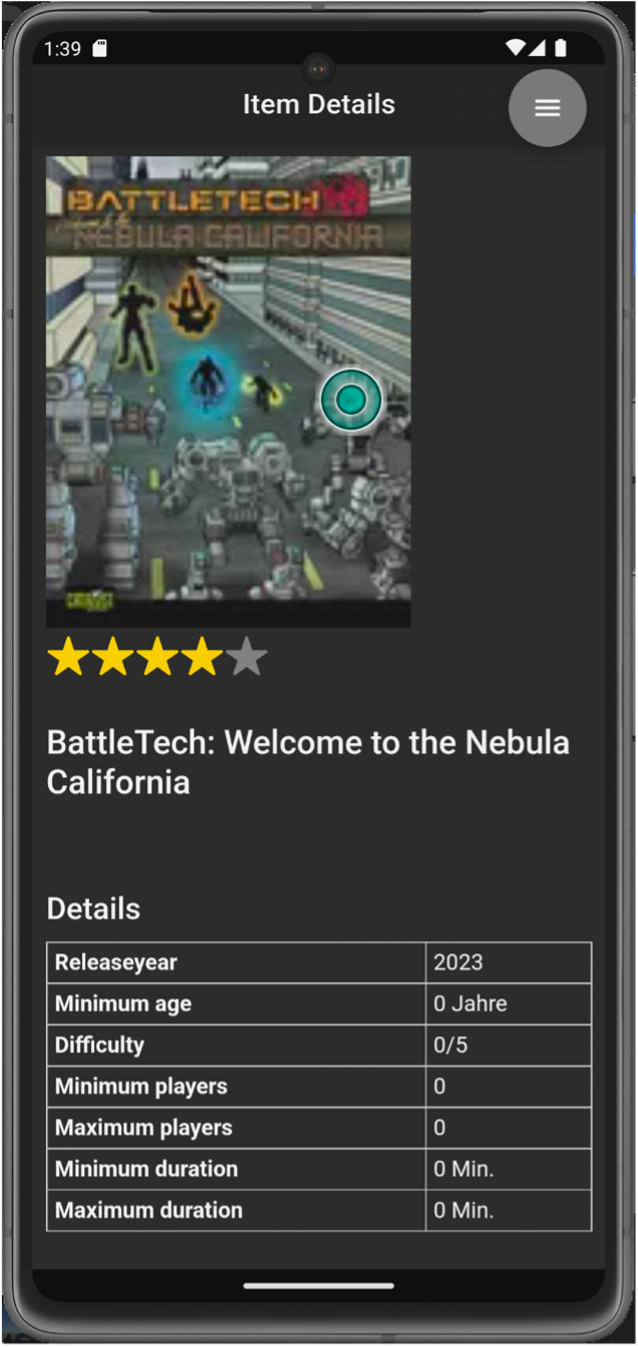
\includegraphics[width=0.4\textwidth]{graphics/infopage.png}
    \caption{Optimierte Detailseite eines Spiels.}
    \label{fig:detailseite}
\end{figure}
\subsection{Unveränderte Elemente}
\begin{enumerate}
    \item \textbf{Grundlegende Struktur:} Die zugrundeliegende Struktur, zu welcher die Hauptnavigation und die Anordnung der Hauptkomponenten gehören, ist im Wesentlichen unverändert geblieben.
    \item \textbf{Kernfunktionen:} Die Kernfunktionen der App, wie die Suche nach Spielen, die Anzeige detaillierter Informationen zu Spielen sowie die Verwaltung von Spielen in Wunschliste und Inventar, haben auch nach Erstellung des Mockups noch Bestand.
\end{enumerate}
\subsection{Fazit}
Die Entwicklung der App vom Mockup bis zum Endprodukt kann als iterativer Prozess angesehen werden, welcher
von ständigen Verbesserungen und Anpassungen geprägt war. Hierbei konnten sich die Kernfunktionen der App
als stabil erweisen, während für Design und Benutzerobefläche kontinuierliche Optimierungspotentiale bestanden (siehe Tab. \ref{fig:optimierung})
In dem Zuge sind auch neue Funktionenen dem Projekt hinzugefügt worden, auch wenn diese nicht im ursprünglichen
Mockup enthalten waren. Ziel war eine kontinuierliche Verbesserung der Benutzererfahrung und Erweiterung des Funktionsumfangs.
\begin{figure}[H]
    \centering
    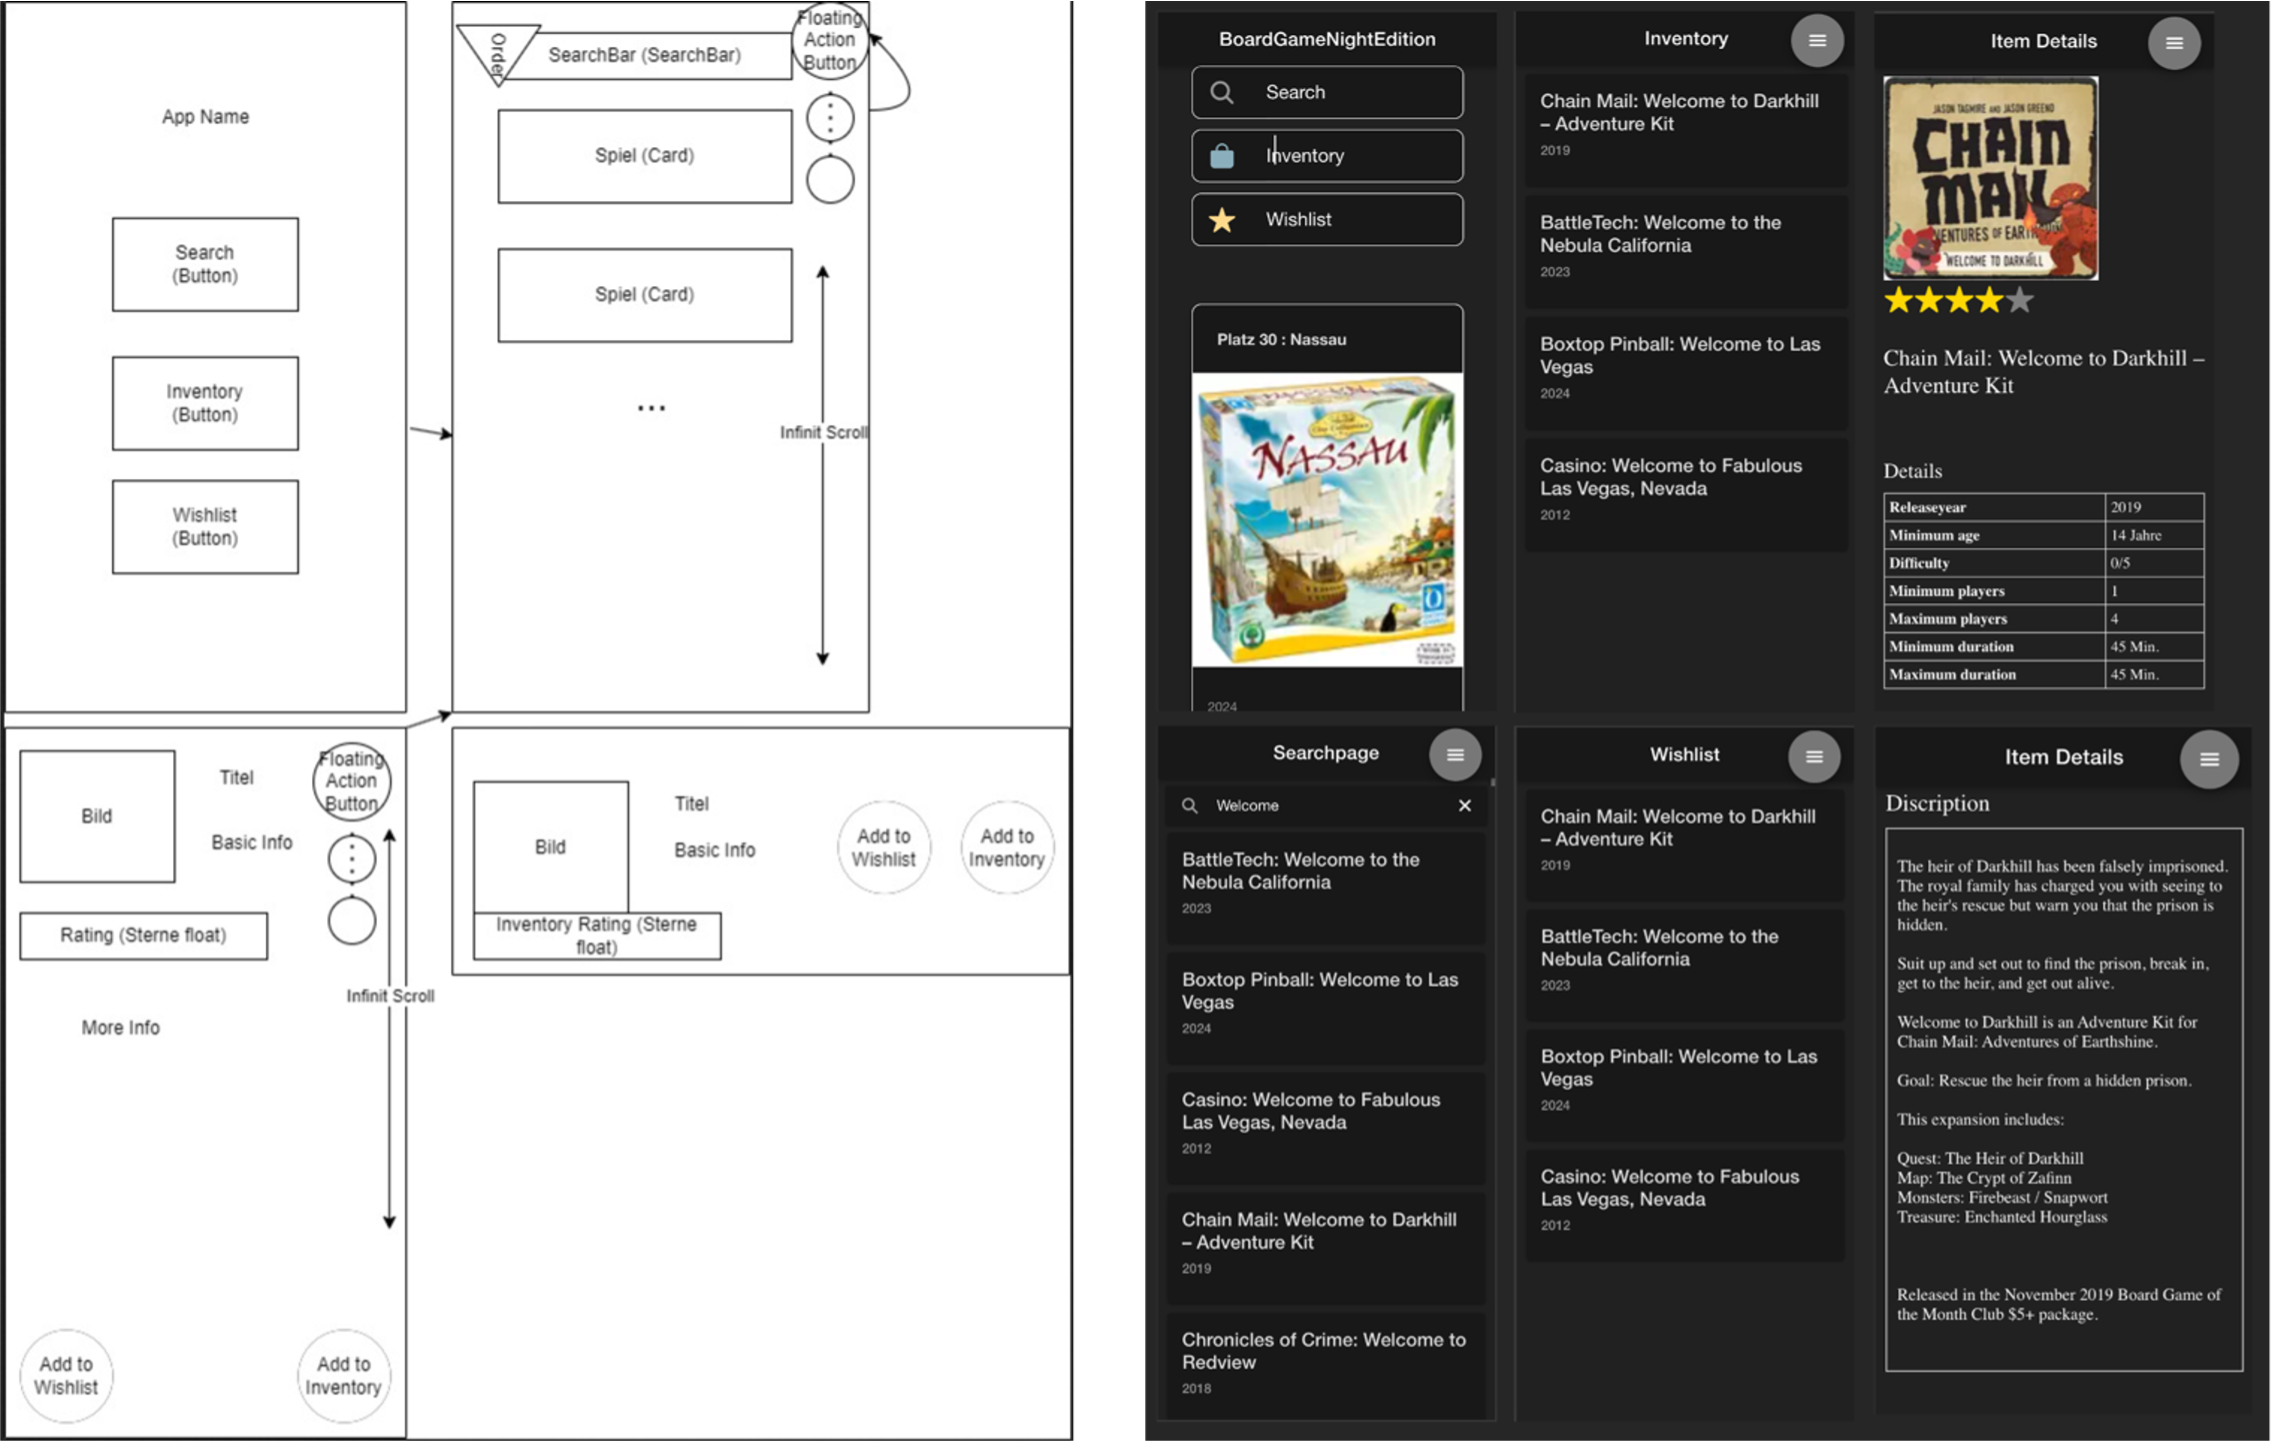
\includegraphics[width=1\textwidth]{graphics/mockup_vergleich.png}
    \caption{Mockup-Vergleich (alt vs. neu).}
    \label{fig:optimierung}
\end{figure}